\documentclass{article}
\title{Example report for the missing 1 dataset}
\usepackage{booktabs} % Required for inserting tables
\usepackage{graphicx} % Required for inserting images
\begin{document}

\maketitle

\section{Introduction}

This is a simple report, which shows how the results of data quality and profiling investigations may be output in plain text, as a webpage or as a Latex document.

Use the paragraph() function to add additional general paragraphs of text.

\section{Results}

\subsection{A section with tables}

Table~\ref{tab:1} shows the number of rows and columns in the dataset.

\begin{table}[h!]
\caption{The size of the dataset.}
\label{tab:1}
\begin{tabular}{lrr}
\toprule
Dataset & Number of rows & Number of columns \\
\midrule
missing 1 & 10000 & 5 \\
\bottomrule
\end{tabular}
\end{table}

Table~\ref{tab:2} shows descriptive statistics for each variable in the dataset.

\begin{table}[h!]
\caption{The data type, an example value and the number of missing values in of each variable.}
\label{tab:2}
\begin{tabular}{lllr}
\toprule
Variable & Data type & Example value & Number of missing values \\
\midrule
A & int64 & 1 & 0 \\
B & float64 & 1.000000 & 1 \\
C & float64 & 1.000000 & 5000 \\
D & float64 & 1.000000 & 9999 \\
E & float64 &  & 10000 \\
\bottomrule
\end{tabular}
\end{table}

Table~\ref{tab:3} shows the same descriptive statistics, but as an image.

\begin{table}[h!]
  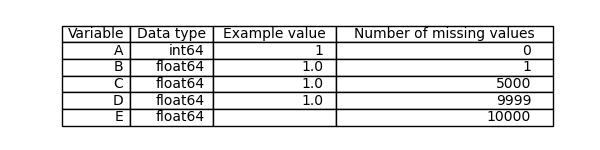
\includegraphics[width=\linewidth]{table_desc_stats.jpg}
  \caption{The data type, an example value and the number of missing values in of each variable.}
  \label{tab:3}
\end{table}

\subsection{A section with figures}

Figure~\ref{fig:1} shows other descriptive statistics for each variable.

\begin{figure}[h!]
  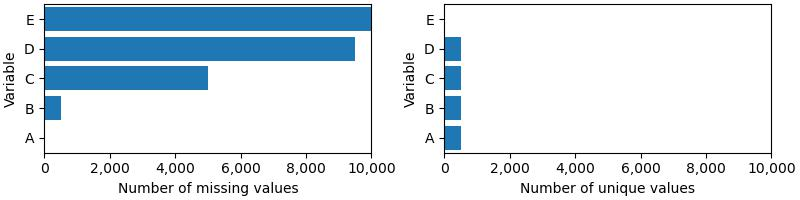
\includegraphics[width=\linewidth]{fig_desc_stats.jpg}
  \caption{The number of values and number of unique values in each variable.}
  \label{fig:1}
\end{figure}

\section{Acknowledgements}

Thank you to A.N. Other for their help. This report was created using the vizdataquality Python package.

\end{document}
